\hypertarget{(chap:capitolo6)}{}
\chapter{Risultati sperimentali}
In questo capitolo andremo a vedere i risultati sperimentali per ogni metodo.
\section{Risultati preprocessing matrici grezze}
Nelle sezione successive andremo a vedere i risultati delle valutazioni di ciascun modello rispetto la metrica $AUC$ e la $NDCG$ con $k\in \{5, 10, 25, 100\}$, in particolare la metrica che riteniamo sia più significativa è la seconda in quanto si basa sul ranking degli item nella lista $TopN$. \\
Per i confronti abbiamo scelto di usare $NDCG$ con $k=25$. Nei seguenti grafici

\subsection{Risultati base}
In questa sezione andremo a vedere i risultati del modello MostPop e del VAECF, che verranno utilizzati come bound per valutare quelli succcessivi. 

\subsubsection{MostPop}
Come detto il modello MostPop restituisce per ogni user la stessa lista di item più popolari.
Andiamo a vedere i risultati per dataset sul validation set:\\

\begin{tabular}{|l|c|cccc|}
    \toprule
    $dataset$ &    $AUC$ &  $NDCG@10$ & $NDCG@100$  & $NDCG@25$ & $NDCG@5$  \\
    \midrule
    macchine & 0.7644 & 0.1263 &   0.2414 &  0.1647 & 0.0920 \\
    ricambi  & 0.3427 &  0.0299 &   0.0732 &  0.0358 & 0.0000 \\
    totale  & 0.2810 &  0.0733 &   0.0811 &  0.0627 & 0.0360 \\

\bottomrule
\end{tabular}

Useremo questi risultati come bound per quelli degli altri modelli (MF,UserKnn), nel caso in cui questi siano migliori si procederà al tuning dei parametri e al calcolo finale dei risultati sul test set.\\
Quelli riportati qui di seguito sono i risultati del MostPop sul test set.\\

\begin{tabular}{|l|c|cccc|}
    \toprule
    $dataset$ &    $AUC$ &  $NDCG@10$ & $NDCG@100$  & $NDCG@25$ & $NDCG@5$  \\
    \midrule
    macchine & 0.7897 &  0.1364 &   0.2610 &  0.1875 & 0.1001 \\
    ricambi  & 0.3924 &  0.0753 &   0.1365 &  0.0793 & 0.0619 \\
    totale  & 0.3101 &  0.0807 &   0.1281 &  0.0866 & 0.0944 \\

\bottomrule
\end{tabular}

\subsubsection{VAECF}
Il modello VAECF è un modello che funziona su rating impliciti, la fase preliminare ha richiesto il tuning dei parametri riportati di seguito:
\begin{itemize}
    \item $n_{int}$ è la dimensione della rappresentazione latente interna, i possibili valori sono $\{5,10,15,20,50\}$;
    \item $n_{hid}$ è il numero di neuroni del layer dell'encoder e del decoder, i valori possibili sono $\{10,20,30,50,100,200\}$;
    \item $f_{act}$ è la funzione di attivazione applicata nei layer nascosti, che può essere una delle seguenti $\{sigmoid, tanh, elu, relu, relu6\}$.
\end{itemize}
\begin{minipage}[H]{0.45\textwidth}
    \begin{tabular}{|l|ccc|}
        \toprule
        $dataset$ &    $n_{int}$ &  $n_{hid}$ & $act\_f$ \\
        \midrule
        macchine & 5 & 30 & relu \\
        ricambi  &	5 & 30 & sigmoid\\
        totale  & 5 & 30 & sigmoid\\
    \bottomrule
    \end{tabular}\\
\end{minipage}
\begin{minipage}[H]{0.55\textwidth}
    Il tuning dei parametri ha portato a considerare tutte le possibili combinazioni dei parametri sopra citati, andiamo a vedere per ogni dataset quali parametri hanno restituito sul validation set i risultati migliori.
\end{minipage}\\

Andiamo a vedere i risultati per dataset sul validation set dopo il tuning dei parametri:\\

\begin{tabular}{|l|c|cccc|}
    \toprule
    $dataset$ &    $AUC$ &  $NDCG@10$ & $NDCG@100$  & $NDCG@25$ & $NDCG@5$  \\
    \midrule
    macchine & 0.8201 & 0.1768 & 0.3032 & 0.2282 & 0.1325	 \\
    ricambi & 0.4773 & 0.0452 & 0.1052 & 0.0643 & 0.0506  \\
    totale  & 0.4190 & 0.0980 & 0.0941 & 0.0741 & 0.1208	 \\
\bottomrule
\end{tabular}\\

Dato che i risultati della tabella precedente sono quelli del validation set su un modello con parametri ottimizzati, non possiamo direttamente usarli per il confronto con 

Vediamo i risultati del modello validato sul test set:\\

\begin{tabular}{|l|c|cccc|}
    \toprule
    $dataset$ &    $AUC$ &  $NDCG@10$ & $NDCG@100$  & $NDCG@25$ & $NDCG@5$  \\
    \midrule
    macchine & 0.8269 &  0.1948 &   0.3301 &  0.2487 & 0.1473 \\
    ricambi  & 0.4930 &  0.0919 &   0.1401 &  0.1075 & 0.0801 \\
    totale  & 0.4343 &  0.0874 &   0.1398 &  0.0964 & 0.0988 \\

\bottomrule
\end{tabular}

\subsection{Risultati MF e UserKnn}
In questa sezione andremo a vedere per ogni tecnica di preprocessing adottata sulle matrici grezze i risultati ottenuti. Cominceremo prima con la tecnica basata su min-max, per proseguire poi con quella ordered-based per concludere con quella basata sui prodotti totali.

\subsubsection{Normalizzazione min-max}
Come spiegato nel capitolo dedicato alle tecniche ora andremo ad osservare i risultati rispetto diversi gruppi di triplette, iniziamo con quelle dal punto di vista globale.

\paragraph{Gruppo globale}
Tutte le triplette sono state considerate nello stesso gruppo, diamo uno sguardo ai risultati ottenuti:

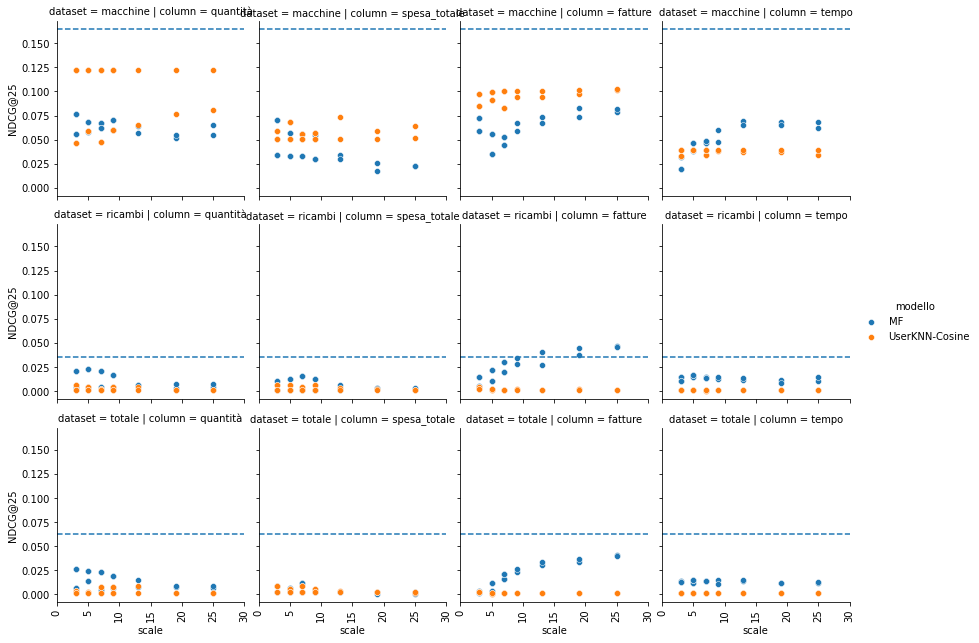
\includegraphics[width=16cm]{figures/risultati_minmax_globale.png}

Nella tabella di grafici sopra riportati possiamo vedere sulle righe i dataset (macchine, ricambi, totale), mentre sulle colonne possiamo vedere le espressioni d'interesse (quantità, )

\paragraph{Gruppi user-based}

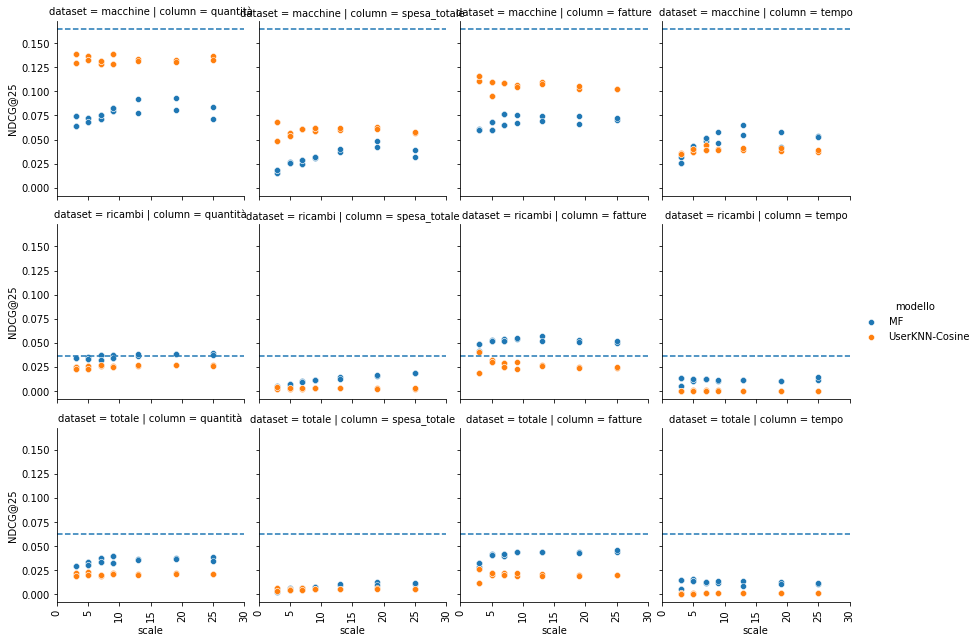
\includegraphics[width=16cm]{figures/risultati_minmax_singolo.png}


\paragraph{Gruppo user-category-based}

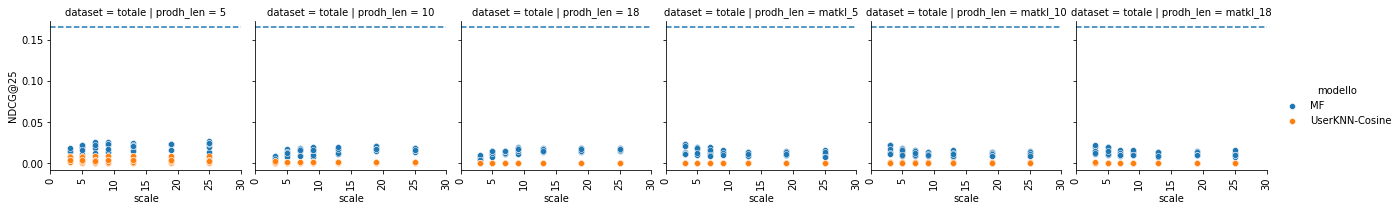
\includegraphics[width=16cm]{figures/risultati_minmax_categoria.png}


\subsubsection{Tecnica ordered-based}

\paragraph{Gruppo globale}
Tutte le triplette sono state considerate nello stesso gruppo, diamo uno sguardo ai risultati ottenuti:

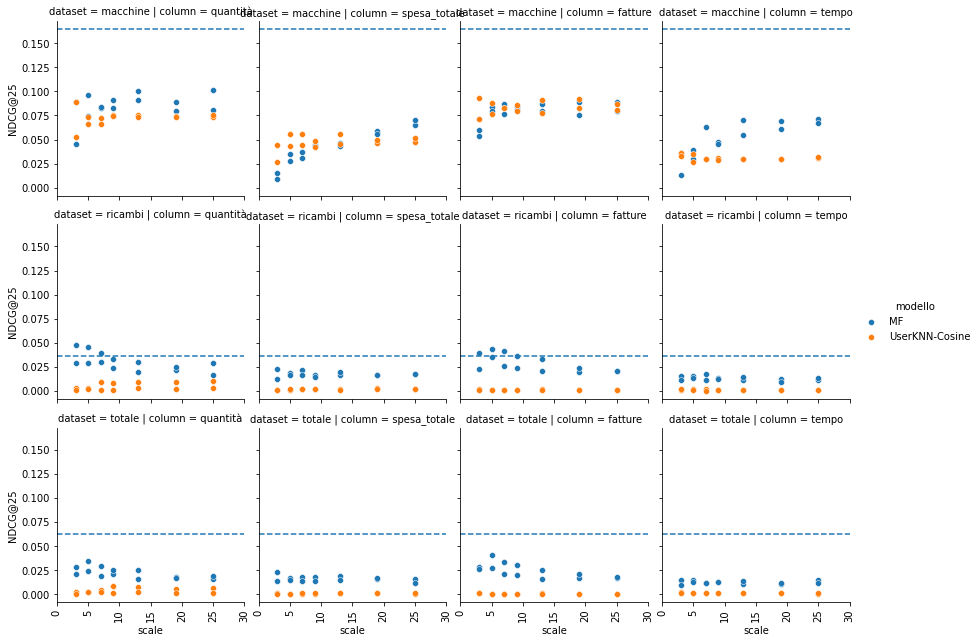
\includegraphics[width=16cm]{figures/risultati_ordered_globale.png}

Nella tabella di grafici sopra riportati possiamo vedere sulle righe i dataset (macchine, ricambi, totale), mentre sulle colonne possiamo vedere le espressioni d'interesse (quantità, )

\paragraph{Gruppi user-based}

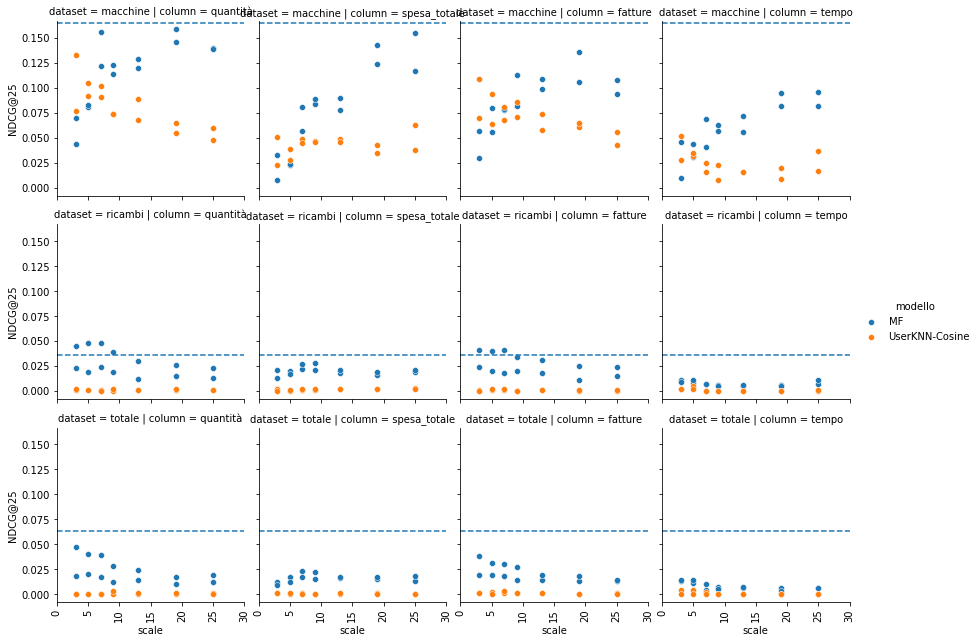
\includegraphics[width=16cm]{figures/risultati_ordered_singolo.png}


\paragraph{Gruppo user-category-based}

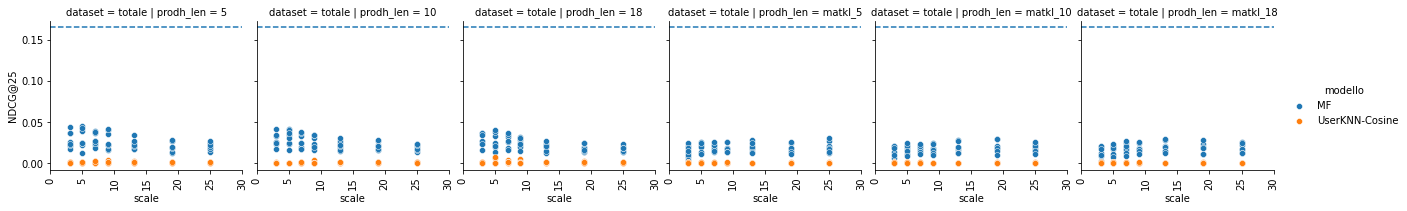
\includegraphics[width=16cm]{figures/risultati_ordered_categoria.png}

\subsubsection{Tecnica product-based}

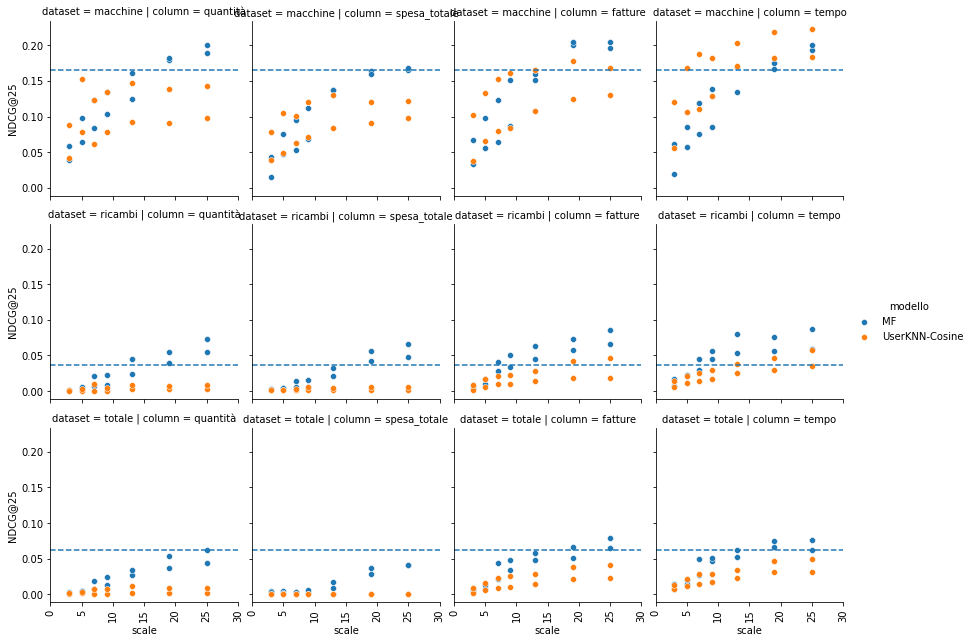
\includegraphics[width=16cm]{figures/prodotto.png}

\section{Risultati matrici grezze combinate}
Vediamo di seguito i risultati delle versioni combinate.

\subsection{Combinazione liste \textit{TopN}}
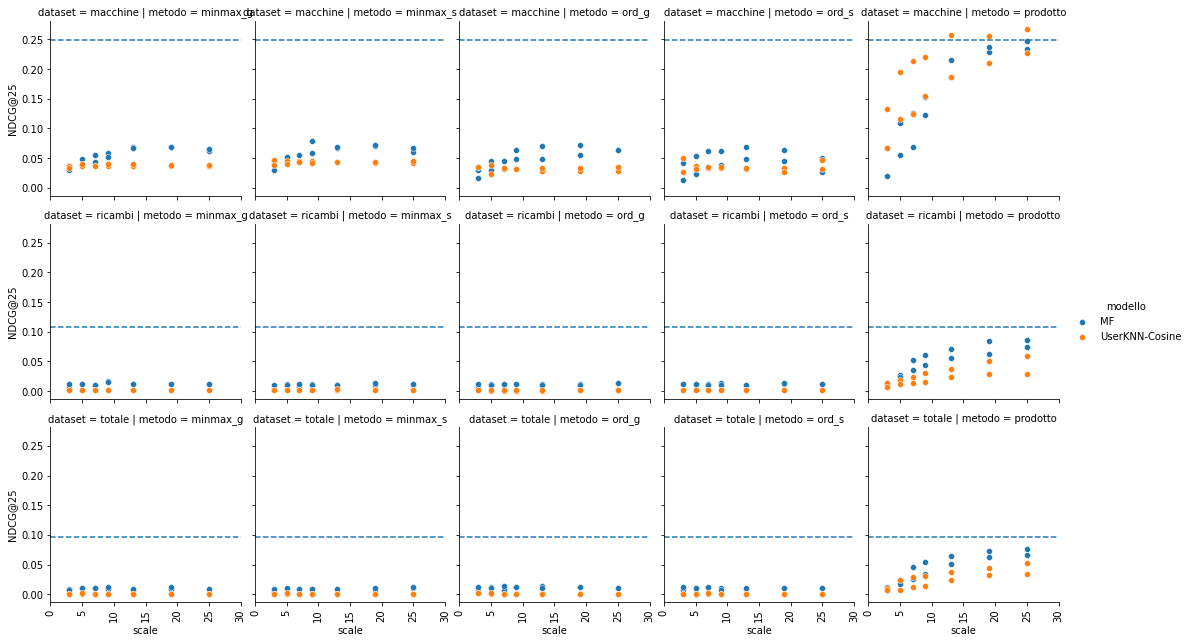
\includegraphics[width=16cm]{figures/comb_1.png}

\subsection{Media matrici dei rating}
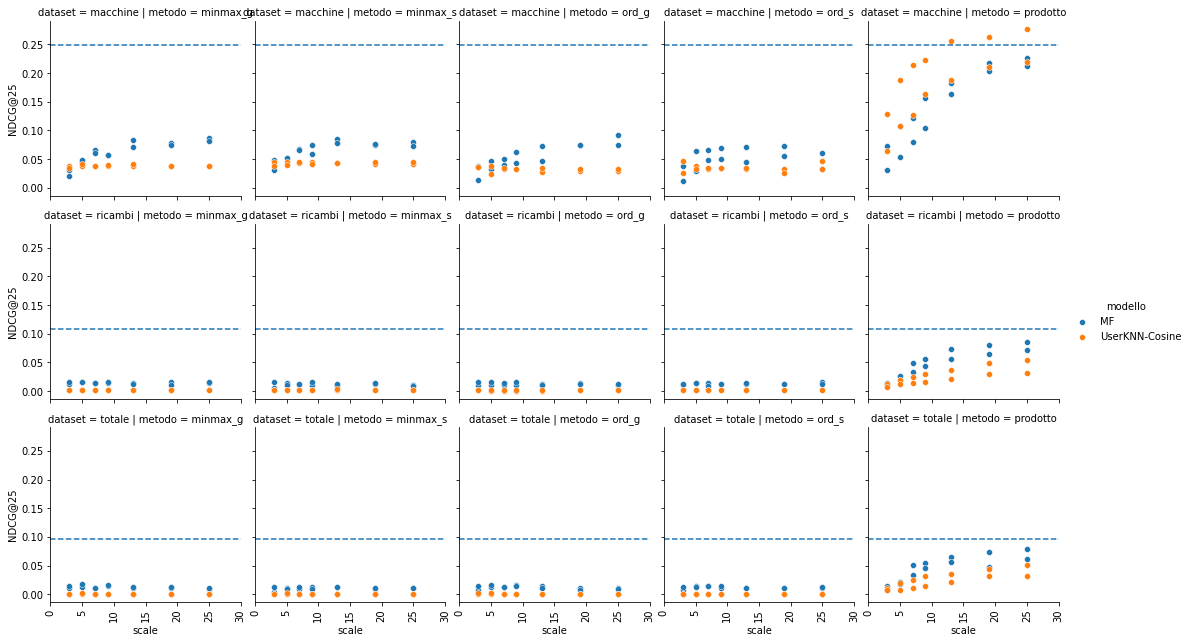
\includegraphics[width=16cm]{figures/comb_2.png}

\section{Esperimenti con approccio next-basket}

